% arara: xelatex: {shell: true}
% arara: biber
% arara: makeglossaries
% arara: xelatex: {shell: true}
% arara: xelatex: {shell: true}
\documentclass[letterpaper,10pt]{article}
\usepackage[margin=1in]{geometry}
\usepackage{hyperref}
\usepackage{graphicx}
\usepackage[justification=centering,font=small,labelfont=bf]{caption}
\usepackage{fancyhdr}
\usepackage{parskip}
\usepackage{fontspec}
\usepackage[toc,nonumberlist]{glossaries}
\usepackage{relsize}
\setmonofont{Inconsolata}[Scale=MatchLowercase]
\defaultfontfeatures{Ligatures=TeX}
\usepackage{xeCJK}
\usepackage{minted}
\usepackage{xcolor}
\definecolor{dsscawpurp}{HTML}{b079b0}
\definecolor{dsscawpurpcap}{HTML}{6c286c}
\usepackage[font={color=dsscawpurpcap},labelfont={sc}]{caption}
\usepackage[backend=biber,
date=iso,
seconds=true,
style=numeric,
bibencoding=utf8,
]{biblatex}

\addbibresource{\jobname.bib}
\usemintedstyle{colorful}
\newenvironment{denseitemize}{
  \begin{itemize}
      \setlength{\itemsep}{0pt}
}{
  \end{itemize}
}
% An attractive 'C++'
\newcommand\CC{C\nolinebreak\hspace{-.05em}\raisebox{.4ex}{\relsize{-3}{\textbf{+}}}\nolinebreak\hspace{-.10em}\raisebox{.4ex}{\relsize{-3}{\textbf{+}}}\hspace{.2em}}

\pagestyle{fancy}
\rhead{
  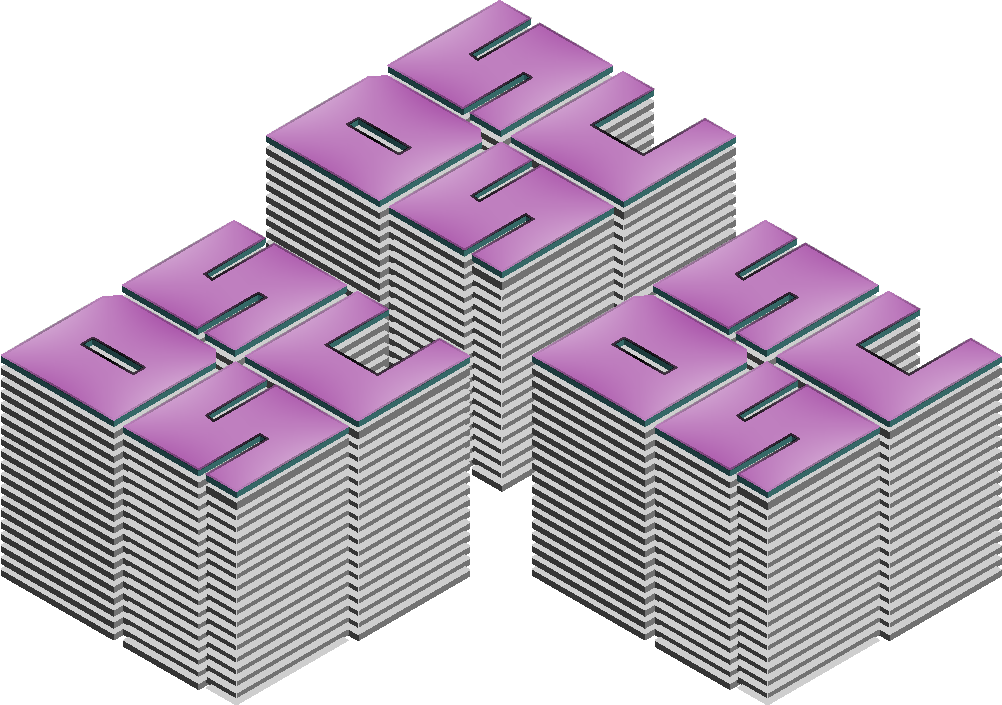
\includegraphics[height=\fontcharht\font`\D,keepaspectratio=true]{../dsscaw-hdr.pdf}
  \textcolor{dsscawpurp}{DSSCAW Technical Report \#004}
}

\title{Hacking the Planet! with Notcurses:\\
A Guide to TUIs and Character Graphics\thanks{
 \href{https://www.dsscaw.com/}{Dirty South Supercomputing of Atlanta, GA.}
}\\
}
\author{Nick Black, Consulting Scientist\\
\texttt{nickblack@linux.com}
}


\makeglossaries
\newglossaryentry{ascii}
{
  name={ANSI X3.4-1968},
  description={A 7-bit character encoding also known as ASCII. Its code set is a proper set of UCS, and its encoding is a proper subset of UTF-8 (but \textit{not} UTF-16, nor UTF-32).}
}

\newglossaryentry{canonical mode}
{
  name={Canonical mode},
  description={A synonym for \gls{cooked mode}},
}

\newglossaryentry{cooked mode}
{
  name={Cooked mode},
description={The default terminal mode under SUSv4 (see \gls{raw mode}).
  The terminal driver buffers input until a newline is entered, while echoing
  it to the screen. Ctrl+C is mapped to \texttt{SIGINT}, Ctrl+\ is mapped to
  \texttt{SIGQUIT}, and Ctrl+Z is mapped to \texttt{SIGTSTP}, and buffered input is flushed
  when these signals are sent. Also known as \gls{canonical mode}.}
}

\newglossaryentry{cdk}
{
  name={CDK},
description={The Curses Development Kit, a widget library developed against the
  Curses specification. It is not distributed as part of NCURSES, though
  both are maintained by Thomas E. Dickey.}
}

\newglossaryentry{cell}
{
  name={Cell},
description={The rectilinear area corresponding to a given text-mode coordinate.
  The analogue of pixels in graphics mode, a cell typically contains more
  pixels along its height than its width. 12 lines of 6 pixels each is not
  unreasonable. A cell can usually represent a grapheme cluster, a foreground
  color, a background color, and some number of attributes, independently
  from surrounding cells.}
}

\longnewglossaryentry{character}
{
  name={Character},
description={One of the most imprecise terms in computer science. The C and \CC
  languages have a data type \texttt{char}, which cannot necessarily hold the
  world's characters. A character is not necessarily a unique concept within
  a character set (see diacritic forms vs. precomposed characters). A
  character does not necessarily correspond to a single column on a display,
  even when using a fixed-width font. A character does not necessarily have a
  visual representation. In a given encoding, all characters are not
  necessarily the same size in a given encoding. A character does not necessarily
  capture the state of the keyboard at some given input.

  In the absence of a coded character set or character encoding for context, a
  character is really nothing more than an identifier with loose syntax:
  \texttt{LATIN CAPITAL LETTER I}. Isn't that a recursive definition? You betcha.

  When I use the word ``character'', I mean either an element of some code set, or
  such an element as encoded by some character encoding. The context ought make
  obvious which meaning is intended.}
}

\newglossaryentry{characterencoding}
{
  name={Character encoding},
description={FIXME}
}

\newglossaryentry{codepoint}
{
  name={Code point},
description={A numerical value within a code space. In and of itself,
  it has neither an associated sequence of bits nor any particular glyph.
  Indeed, a code point might correspond to some non-printable control.}
}

\newglossaryentry{codeset}
{
  name={Code set},
description={A set of abstract characters, each having a name and a code
  point. ISO/IEC 10646 specifies over 100,000 abstract characters as the
  Universal Coded Character Set (UCS). This is smaller than its corresponding
  code space by about two orders of magnitude. Also known as a \textbf{coded character set}.}
}

\newglossaryentry{codespace}
{
  name={Code space},
description={A numerical range spanning all the code points of a code set.
  The Unicode code space (as of Unicode 13) is made up of 17 contiguous
  planes of 65,536 contiguous code points each, for a size of $17*2^{16}$.}
}

\newglossaryentry{console}
{
  name={Console},
description={Though sometimes used synonymously with ``terminal'', console almost
  always refers to text-based environments on personal computers. On Linux
  x86 machines, this could mean a serial terminal, an AT keyboard and a VGA
  in 80x25 text mode, a USB keyboard with a UEFI framebuffer, or any number
  of other things. When I use ``console'', I mean terminals outside of a GUI
  context.}
}

\newglossaryentry{curses}
{
  name={Curses},
description={The X/OSI specification of an API for optimized cursor routines. It
  was most recently ratified as part of the January 2018 Single UNIX
  Specification version 4 administrative rollup, aka ``susv4-2018''. NCURSES is
  an implementation of Curses (plus extensions). Notcurses is not.}
}

\newglossaryentry{cursor}
{
  name={Cursor},
description={Both the location where output will next be written, and possibly
  a visual indication of that location.}
}

\newglossaryentry{dialog}
{
  name={dialog},
description={An NCURSES-based application for TUI modal dialogs.}
}

\newglossaryentry{egc}
{
  name={Extended Grapheme Cluster},
description={FIXME }
}

\newglossaryentry{isoiec2022}
{
  name={ISO/IEC 2022},
description={FIXME }
}

\newglossaryentry{isoiec10646}
{
  name={ISO/IEC 10646},
description={``Information technology — Universal Coded Character Set (UCS)''.}
}

\newglossaryentry{keyboard}
{
  name={Keyboard},
description={An input device primarily used to select from a set of
  characters. These characters might or might not correspond to elements in
  the active encoding. Unlike pointers, keyboards do not indicate position.}
}

\newglossaryentry{ncurses}
{
  name={NCURSES},
description={An implementation of X/OSI Curses (plus extensions) maintained by
  Thomas E. Dickey under the auspices of the Free Software Foundation.
  Installed on just about every currently-running UNIX system, it is a
  venerable, proven library, and the foundation of a great many applications.}
}

\newglossaryentry{newt}
{
  name={Newt},
description={A minimal TUI library written atop slang, providing the foundation
  for \texttt{whiptail}. It is not a Curses implementation.}
}

\newglossaryentry{noncanonical}
{
  name={Non-canonical mode},
description={A synonym for \gls{raw mode}.}
}

\newglossaryentry{notcurses}
{
  name={Notcurses},
description={The baddest character graphics/TUI library in town.}
}

\newglossaryentry{pointer}
{
  name={Pointer},
description={An input device primarily used to indicate position. It
  corresponds with one cell at any given time, which might or might not be
  independent of the cursor. There can be more than one pointer. Like a
  keyboard, pointers typically have (usually far fewer) distinct buttons.}
}

\newglossaryentry{pgroup}
{
  name={Process group},
description={A set of processes sharing the same PGID. When the terminal
  generates a signal for a process (e.g. \texttt{SIGINT} in response to Ctrl+C), it
  sends the signal to all processes in that process group. Of the process
  groups making up a session, only one is the foreground process group.
  Attempts to perform terminal I/O by session processes outside the foreground
  process group will result in \texttt{SIGTTIN} or \texttt{SIGTTOU}.}
}

\longnewglossaryentry{pseudoterminal}
{
  name={Pseudoterminal},
description={``A pair of virtual character devices that provide a
  bidirectional communication channel. One end of the channel is called the
  master; the other end is called the slave. The slave end of the
  pseudoterminal provides an interface that behaves exactly like a classical
  terminal. A process that expects to be connected to a terminal, can open
  the slave end of a pseudoterminal and then be driven by a program that has
  opened the master end. Anything that is written on the master end is
  provided to the process on the slave end as though it was input typed on a
  terminal.'' (\texttt{pty(7)} Linux Programmer's Manual page)

 Pseudoterminals are used by terminal emulators and interactive SSH
  connections. They are essentially buffers with some basic transformation
  capabilities. Ctrl-C is turned into \texttt{SIGINT} by the pseudoterminal device,
  and it handles relevant \texttt{ioctl()}s.}
}

\newglossaryentry{raw mode}
{
  name={Raw mode},
description={A collection of behaviors differing from \gls{cooked mode}. Noticeably,
  the terminal driver no longer buffers input or generates signals.}
}

\longnewglossaryentry{terminal}
{
  name={Terminal},
description={In the abstract, a means for entering data into a computer
  (typically involving a keyboard, and often a pointing device), and a means
  for displaying that conmputer's output. In the concrete, electromechanical
  devices for doing the same. I use ``terminal'' in the abstract sense
  throughout this book, but both meanings are in common use:

  \begin{denseitemize}
  \item I pull my chair up to my desk and \textit{engage my terminal}.
  \item I press Meta+F1 and \textit{bring up a terminal}.
  \end{denseitemize}

 Only the mad might refer to a physical device as a terminal emulator.}
}

\longnewglossaryentry{terminalemulator}
{
  name={Terminal emulator},
description={A program in a GUI environment providing a
  two-dimensional array of cells. A terminal emulator differs from a
  framebuffer/canvas in that each of these cells contains rendered (and
  possibly stylized) font glyphs, as opposed to a single pixel. Terminal
  emulator processes are connected to the slave ends of pseudoterminals.

 The pure character graphics environment of e.g. Linux or FreeBSD outside
  of X11 or Wayland is technically a terminal emulator, but almost always
  referred to as a ``console''. When I say ``terminal emulator'' in this book,
  I do not mean to include consoles.}
}

\newglossaryentry{termcap}
{
  name={termcap},
description={A deprecated terminal capability database, superseded by \gls{terminfo}.}
}

\newglossaryentry{terminfo}
{
  name={terminfo},
description={A database describing terminals and their capabilities. It is
  primarily indexed by terminal name, yielding an entry covering several
  hundred capabilities. These capabilities are then indexed by name. A
  terminal environment is responsible for setting the \texttt{TERM} environment
  variable to the correct primary terminfo index. termcap has been
  deprecated by the introduction of terminfo, which is superior in every way.}
}

\newglossaryentry{termios}
{
  name={termios},
description={A POSIX API and data structure for working with arbitrary terminals.
  These functions all start with \texttt{tc} or \texttt{cf}, and control low-level behavior.}
}

\newglossaryentry{ucs2}
{
  name={UCS-2},
description={A fixed-length encoding of the Basic Multilingual Plane. Each
  character is encoded to a single 16-bit code unit, for a total of 2 bytes
  per encoded character. UCS-2 cannot encode all of UCS, and is infrequently
  used. An amendment to ISO/IEC 10646 extended UCS-2 to UTF-16.}
}

\newglossaryentry{ucs4}
{
  name={UCS-4},
description={A fixed-length encoding of UCS to 32-bit code units. RFC 3629
  restricted UCS-4 to UTF-32.}
}

\newglossaryentry{unicode}
{
  name={Unicode},
description={UCS as defined by ISO/IEC 10646 (which Unicode inducts), plus
  rules on how to use that code set. Unicode is defined by the Unicode
  Consortium.}
}

\newglossaryentry{utf1}
{
  name={UTF-1},
description={An early garbage form of UTF-8. ISO 10646 Annex G, since deprecated.
  Unfortunately, the page might not yet have been ripped out at your local
  library. Don't use UTF-1.},
}

\newglossaryentry{utf8}
{
  name={UTF-8},
description={FIXME}
}

\newglossaryentry{utf16}
{
  name={UTF-16},
description={A variable-length encoding of UCS. Each character is encoded to
  either one or two 16-bit code units, for a total of 2 or 4 bytes per
  encoded character. There's very little good about UTF-16, and it ought
  neither be purchased, nor accepted as a gift. Perhaps not coincidentally,
  it is the internal encoding of both Microsoft Windows and Java.}
}

\newglossaryentry{utf32}
{
  name={UTF-32},
description={A fixed-length encoding of UCS. Each character is encoded to a
  single 32-bit code unit, for a total of 4 bytes per encoded character.}
}

\newglossaryentry{virtualterm}
{
  name={Virtual terminal},
description={Some consoles multiplex multiple instances. Each is
  typically referred to as a virtual terminal. I have never heard anyone
  refer to the multiple tabs of a terminal emulator as ``virtual terminals'',
  and would look at them strangely if I did.}
}

\newglossaryentry{whiptail}
{
  name={whiptail},
description={An application for providing TUI modal dialogs, similar to \texttt{dialog}. It is written using Newt.}
}

\newglossaryentry{widechar}
{
  name={Wide character},
  description={This has at least two distinct meanings:
\begin{denseitemize}
\item \texttt{wchar\_t}: A data type in C and \CC. FIXME
\item \textbf{Wide East Asian characters}: FIXME
\end{denseitemize}
}
}

%%%%%%%%%%%%%%%%%%%%%%%%%%%%%%%%%%%%%%%%%%%%%%%%%%%%%%%%%%%%%%%%%%%%%%%%
\begin{document}
%%%%%%%%%%%%%%%%%%%%%%%%%%%%%%%%%%%%%%%%%%%%%%%%%%%%%%%%%%%%%%%%%%%%%%%%
\date{Feb 14, 2020}
\maketitle
\thispagestyle{fancy}
\date{}
\vspace{1in}
\begin{center}
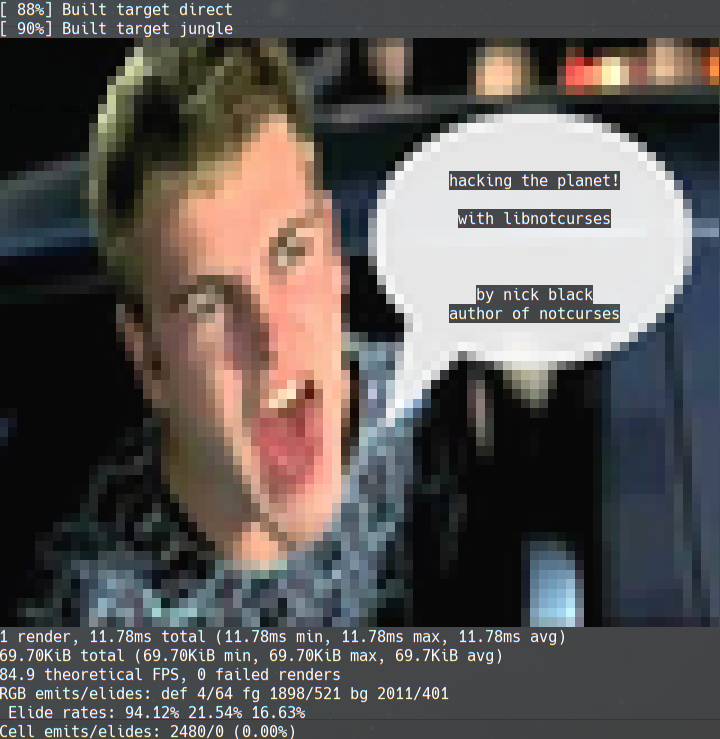
\includegraphics[width=.75\linewidth]{htp-with-notcurses.png}
\end{center}
%%%%%%%%%%%%%%%%%%%%%%%%%%%%%%%%%%%%%%%%%%%%%%%%%%%%%%%%%%%%%%%%%%%%%%%%

\clearpage

\tableofcontents

\clearpage

\section{Introduction}

I implemented Notcurses in the winter of 2019 after having a few patches
rejected from NCURSES (the first commit was pushed 2019-11-16, and I started
writing this manuscript 2020-02-12, following the 1.1.8 release). It proved to
be seductive as hell, and it was only with difficulty that I tore myself away
following three months of hard work. By that time, Notcurses subsumed most
functionality of NCURSES, adding a great deal more. The project had three
major goals:

\begin{denseitemize}
\item  to provide NCURSES-like functionality with 24-bit color, safety in the
    prescence of multithreading, and full Unicode support,
\item to reduce the amount of boilerplate code necessary for the UIs of my
    TUI applications, including \textit{growlight} and \textit{omphalos}, and
\item to portably facilitate the most vivid character graphics possible.
\end{denseitemize}

Many people asked why such a thing was useful. My usual response was that
numerous devices don't present a bitmap interface, that X11 GUIs run remotely
over SSH are effectively unusable, that plenty of machines don't have a GUI
environment installed, and that Sixel isn't well-supported across different
terminal emulators. It seems impossible in an age of gigatransistor graphics
cards, but the text environment still presents perceivably less latency
than most GUI toolkits. That I was able to remove thousands of lines
of NCURSES code from my applications was a nice side benefit.

In truth, the main reasons were that it was fun, and I wanted to see how far
I could push it.

As I write this, Notcurses is present in Arch's AUR, and is awaiting promotion
into the Debian Incoming queue. Written as a C core, it enjoys \CC, Python, and
Rust wrappers. I have submitted it as a backend to NEStopia and RetroArch, and
intend to integrate it into Mesa as an OpenGL backend. So long as one can live
with the limited resolution available when a screen is divided into rectangular
cells, it can handle any graphics thrown at it. I hope to see it displace
NCURSES as the go-to character graphics library for new applications (there is
little value in porting existing applications to Notcurses, since an unchanged
application wouldn't take advantage of its advanced features).

While the X/OSI Curses specification is unlikely to ever go away (nor should
it, as a lowest-common-denominator interface to devices Notcurses is unlikely
to ever support), I believe Notcurses to present a superior API and
implementation for modern TUI applications.

The console ain't dead! Hack on, hax0rs.

\vspace{.5in}

\begin{flushright}
  \textit{---February 2020, Atlanta}
\end{flushright}

\vspace{1in}

\begin{center}
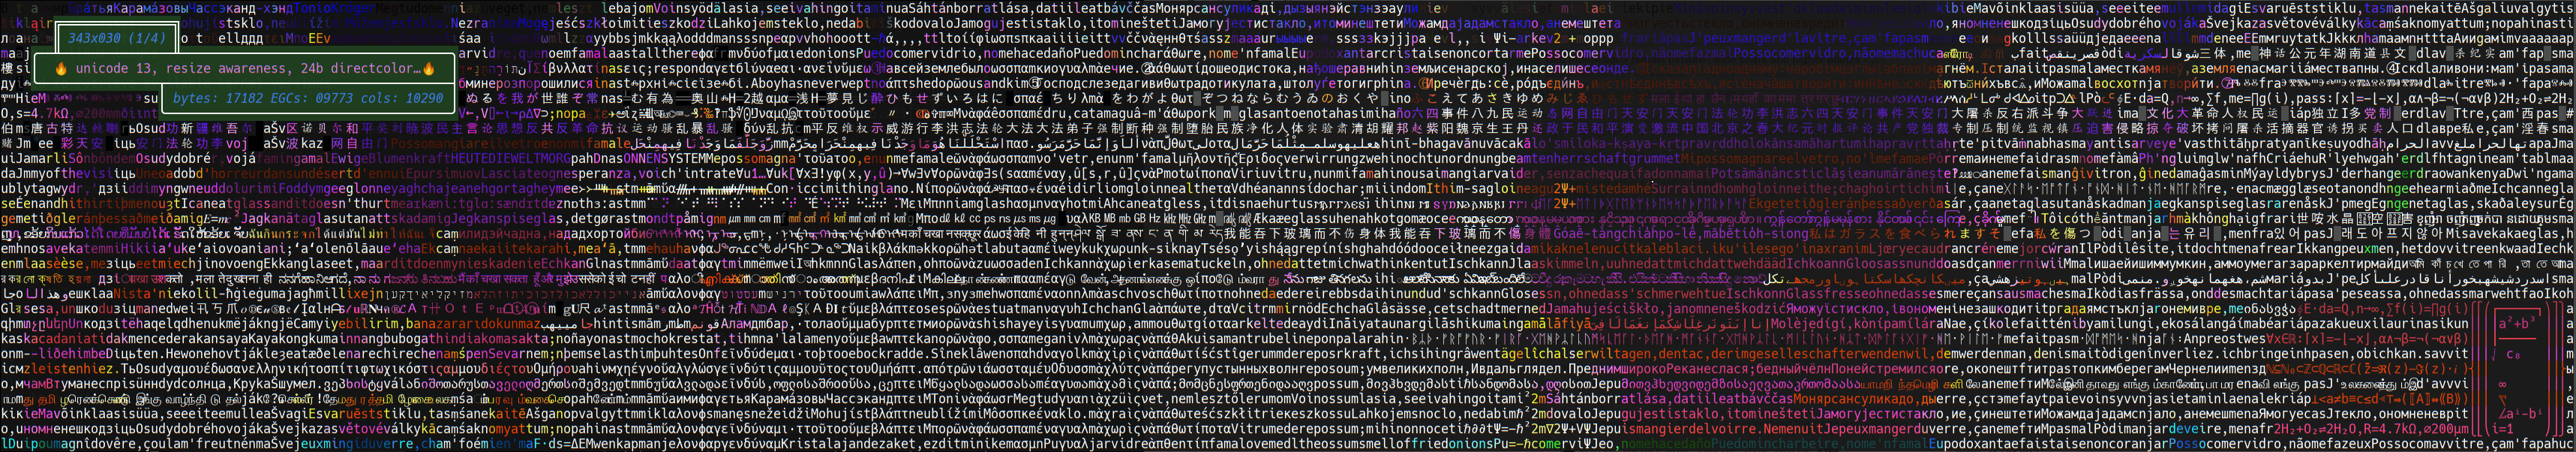
\includegraphics[width=1\linewidth]{media/widechars.png}
\end{center}

\newpage

\section{A brief history of character graphics}
\subsection{The Curses API}

\newpage

\section{Using Direct mode with standard I\/O}

Many tools don't intend to be full-screen TUI applications, but instead
implement that purest of UNIX interfaces: newline-delimited text, oblivious
to screen geometry, capable of being fed as input to other, similar programs.
For such tools, the full Notcurses capabilities are neither necessary nor
desirable. These programs are typically non-interactive: humans might peruse
their outputs and prepare their inputs, but they effectively run as a batch
task.

Such tools might still want to colorize and otherwise style their output, at
least when being output to a terminal. This can be accomplished using the
\texttt{ncdirect} subset of Notcurses, and is known as \textit{direct mode}. Direct
mode functionality should not usually be mixed with other Notcurses calls.
Unlike full Notcurses, there is no explicit rendering step in direct mode, and
it is intended to be mixed among other use of standard I/O. Essentially, direct
mode ``styles your \texttt{printf()}s.'' Similarly to full Notcurses, direct mode
requires a valid and correct terminfo database entry, supplied via either the
\texttt{termtype} parameter to \texttt{notcurses\_directmode()} or the \texttt{TERM} environment
variable. It does \textit{not}, however, require any particular encoding nor
even a call to \texttt{setlocale()} (full Notcurses requires a properly-configured
ASCII or UTF-8 locale).

Enter direct mode via a call to \texttt{notcurses\_directmode()} with a successful
return of a non-\texttt{NULL} pointer to \texttt{struct ncdirect}:

\begin{listing}[ht]
\begin{minted}{C}
// Initialize a direct-mode notcurses context on the connected terminal at 'fp'.
// 'fp' must be a tty. You'll usually want stdout. Direct mode supportes a
// limited subset of notcurses routines which directly affect 'fp', and neither
// supports nor requires notcurses_render(). This can be used to add color and
// styling to text in the standard output paradigm. Returns NULL on error,
// including any failure initializing terminfo.
struct ncdirect* notcurses_directmode(const char* termtype, FILE* fp);
\end{minted}
\end{listing}

It is typical to invoke this function as \texttt{notcurses\_directmode(NULL, stdout)}.
In this case, the terminal type must be present in the \texttt{TERM} environment
variable (this should have been done by the terminal). The buffering and
blocking status of \texttt{fp} will not be changed. \texttt{NULL} is returned for any number
of possible errors. Otherwise, the \texttt{struct ncdirect} is ready to go, and should
be cleaned up with \texttt{ncdirect\_stop()}:

\begin{listing}[ht]
\begin{minted}{C}
// Release 'nc' and any associated resources. 0 on success, non-0 on failure.
int ncdirect_stop(struct ncdirect* nc);
\end{minted}
\end{listing}

Between these two calls, inject stylizing control codes into the \texttt{FILE*} with
the following API:

\begin{listing}[ht]
\begin{minted}{C}
int ncdirect_bg_rgb8(struct ncdirect* n, unsigned r, unsigned g, unsigned b);
int ncdirect_fg_rgb8(struct ncdirect* n, unsigned r, unsigned g, unsigned b);
int ncdirect_fg(struct ncdirect* n, unsigned rgb);
int ncdirect_bg(struct ncdirect* n, unsigned rgb);
int ncdirect_fg_default(struct ncdirect* n);
int ncdirect_bg_default(struct ncdirect* n);
int ncdirect_styles_set(struct ncdirect* n, unsigned stylebits);
int ncdirect_styles_on(struct ncdirect* n, unsigned stylebits);
int ncdirect_styles_off(struct ncdirect* n, unsigned stylebits);
int ncdirect_clear(struct ncdirect* n);
\end{minted}
\end{listing}

While direct mode does not offer any means for moving the cursor in
two-dimensional space, it does provide helpers for determining the terminal
geometry:

%\begin{listing}[ht]
\begin{minted}{C}
int ncdirect_dim_x(const struct ncdirect* nc);
int ncdirect_dim_y(const struct ncdirect* nc);
\end{minted}
%\end{listing}

\subsection{Example: presenting \textit{\textcolor{blue}{House} of Leaves}}

Mark Z. Danielewski's 2000 experimental novel \textit{House of Leaves} prints each 
instance of the word \textcolor{blue}{house} in blue, even when it is a subword:

\begin{center}
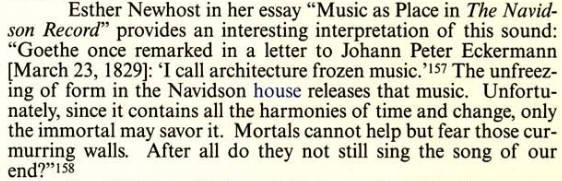
\includegraphics[width=.5\linewidth]{house-blue.png}
\end{center}

We can easily write code to reproduce this effect for standard input and output:

\begin{listing}[ht]
\inputminted[fontsize=\scriptsize]{C}{code/hol-formatter.c}
\end{listing}

This works as expected:

\begin{center}
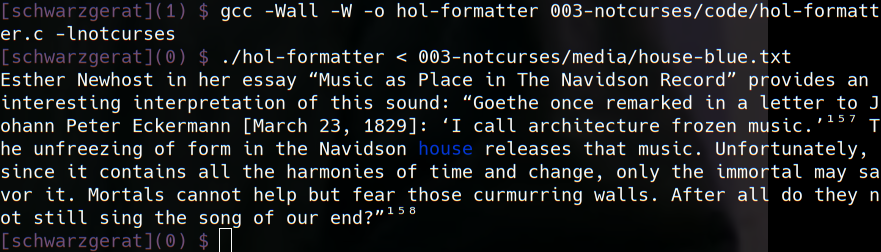
\includegraphics[width=.75\linewidth]{hol-formatted.png}
\end{center}

There are a few things worth noting about the code above. First, observe how
much of the logic is devoted to checking and propagating errors! It is, perhaps
contrary to common expectations, necessary to check the results of e.g.
\texttt{print()} in a reliable program (what happens if we're redirect to a file, and
the disk is full?). A language making use of exceptions would reduce if not
eliminate this nonsense.

We don't switch from blue to some random color, because we don't know the
background color of the terminal. Hard to believe as it is, some people don't
favor a dark terminal background. If the terminal background was white, and we
had just used e.g. \texttt{ncdirect\_fg(n, 0xffffff)}, text following
``\textcolor{blue}{house}'' would be invisible.

One might observe that a user with a blue background will have invisible ``house'' text.
This is true, and there's no great solution to it. It is not generally possible to
discover the RGB values of the default colors. I suppose all one can do is rest easy,
knowing that people with chromatic backgrounds deserve whatever happens to them.

\subsection{Example: colorizing a dumb game}

Imagine we've written the following guessing game:

\begin{listing}[ht]
\inputminted[fontsize=\scriptsize]{C}{code/hilostdio.c}
\end{listing}

The correct approach is binary search, and for an $N$-bit long, we expect to
guess the number in no more than $N$. Let's color the output to indicate how
bad of a guess was offered. We'll use blue for low guesses, red for high
guesses, and break the 256 shades of each (assuming the other two components
to be fixed) uniformly across the $N$ levels of logarithmic
distance\footnote{Gamma correction?}. If we wanted to do this without direct
use of RGB color, we'd either need accept fewer shades, or be forced to
reprogram the palette.

Stepping through the orders of magnitude, we get the expected gradient. Were
we to actually play, the response would converge to a balanced, strong green
as we approached the correct answer.

\begin{center}
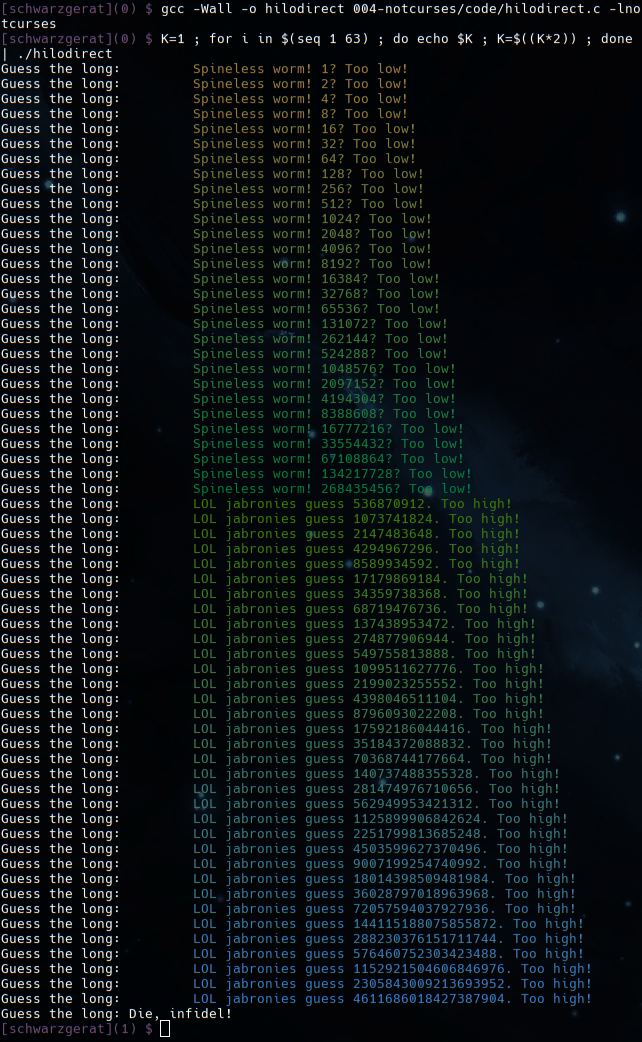
\includegraphics[width=.75\linewidth]{media/hilodirect.png}
\end{center}
\newpage


%%%%%%%%%%%%%%%%%%%%%%%%%%%%%%%%%%%%%%%%%%%%%%%%%%%%%%%%%%%%%%%%%%%%%%%%
\section{A simple notcurses render\/event loop}
\newpage

%%%%%%%%%%%%%%%%%%%%%%%%%%%%%%%%%%%%%%%%%%%%%%%%%%%%%%%%%%%%%%%%%%%%%%%%
\section{Using ncplanes}
\newpage

%%%%%%%%%%%%%%%%%%%%%%%%%%%%%%%%%%%%%%%%%%%%%%%%%%%%%%%%%%%%%%%%%%%%%%%%
\section{Styling with colors and attributes}
\newpage

%%%%%%%%%%%%%%%%%%%%%%%%%%%%%%%%%%%%%%%%%%%%%%%%%%%%%%%%%%%%%%%%%%%%%%%%
\section{Lines, boxes, and fills}
\newpage

%%%%%%%%%%%%%%%%%%%%%%%%%%%%%%%%%%%%%%%%%%%%%%%%%%%%%%%%%%%%%%%%%%%%%%%%
\section{Collecting and dispatching input}
\newpage

%%%%%%%%%%%%%%%%%%%%%%%%%%%%%%%%%%%%%%%%%%%%%%%%%%%%%%%%%%%%%%%%%%%%%%%%
\section{Multimedia (images and videos)}
\newpage

%%%%%%%%%%%%%%%%%%%%%%%%%%%%%%%%%%%%%%%%%%%%%%%%%%%%%%%%%%%%%%%%%%%%%%%%
\section{Unicode, UTF-8, and multicolumn glyphs}
\newpage

%%%%%%%%%%%%%%%%%%%%%%%%%%%%%%%%%%%%%%%%%%%%%%%%%%%%%%%%%%%%%%%%%%%%%%%%
\section{UI widgets}
\newpage

\newpage
%%%%%%%%%%%%%%%%%%%%%%%%%%%%%%%%%%%%%%%%%%%%%%%%%%%%%%%%%%%%%%%%%%%%%%%%
\glsaddallunused
\printglossary[title={Glossary of terms \textit{as used in this manuscript}}]
%%%%%%%%%%%%%%%%%%%%%%%%%%%%%%%%%%%%%%%%%%%%%%%%%%%%%%%%%%%%%%%%%%%%%%%%
\printbibliography
%%%%%%%%%%%%%%%%%%%%%%%%%%%%%%%%%%%%%%%%%%%%%%%%%%%%%%%%%%%%%%%%%%%%%%%%
\vfill
\begin{center}
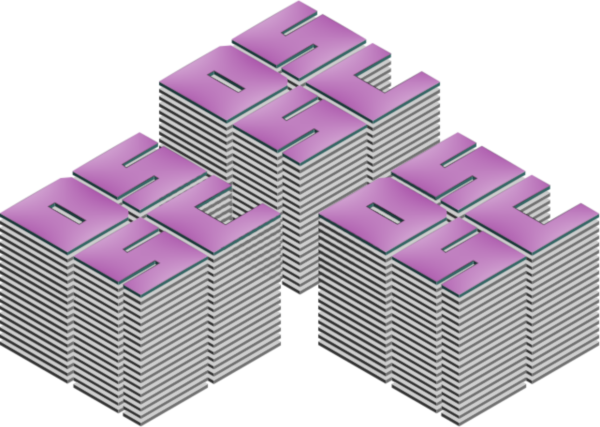
\includegraphics[width=.4\linewidth]{../common/dsscaw-purp-scaled.png}

\includegraphics[width=.5\linewidth]{../common/south.png}
\end{center}
\end{document}
